\section{Постановка задачи}
\subsection{Задача}
Задачей в проекте было создание алгоритма для наблюдением за эволюцией ледового канала. Фактически алгоритм должен выдавать ширину канала на 
некотором удалении от кормы ледокола. Из-за недостатка ресурсов, сжатых сроков и особенностей связанных с деплоем на эксплуатирующийся ледокол задача была поделена на две части:
\begin{enumerate}
    \item Реализация при помощи тех технических средств и программного обеспечения, которые уже есть на ледоколе
    \item Реализация более точного алгоритма с возможностью использовать дополнительное программное обеспечение и, возможно, дополнительные технические средства.
\end{enumerate}

Было решено решать более общую задачу. Вместо ширины канала искать маску канала и уже по ней определять ширину и другие параметры.

На ледоколе были установлены следующие устрйства:
\begin{enumerate}
    \item Камера с разрешением 1920*1080
    \item Лидар Livox Avia
    \item Компьютер для расчетов (без видеокарты) 
\end{enumerate}

Для работы алгоритма было решено использовать снимки камеры, так как эффективная дальность лидара в детектировании ледовой поверхности не превышает 100 метров, 
в то время как камера способна ``видеть'' более, чем на километр. Однако у камеры есть другая проблема, ночные снимки камеры практически невозможно анализировать.

\begin{figure}[htbp]
    \centering
    \subfloat[Дневной снимок]{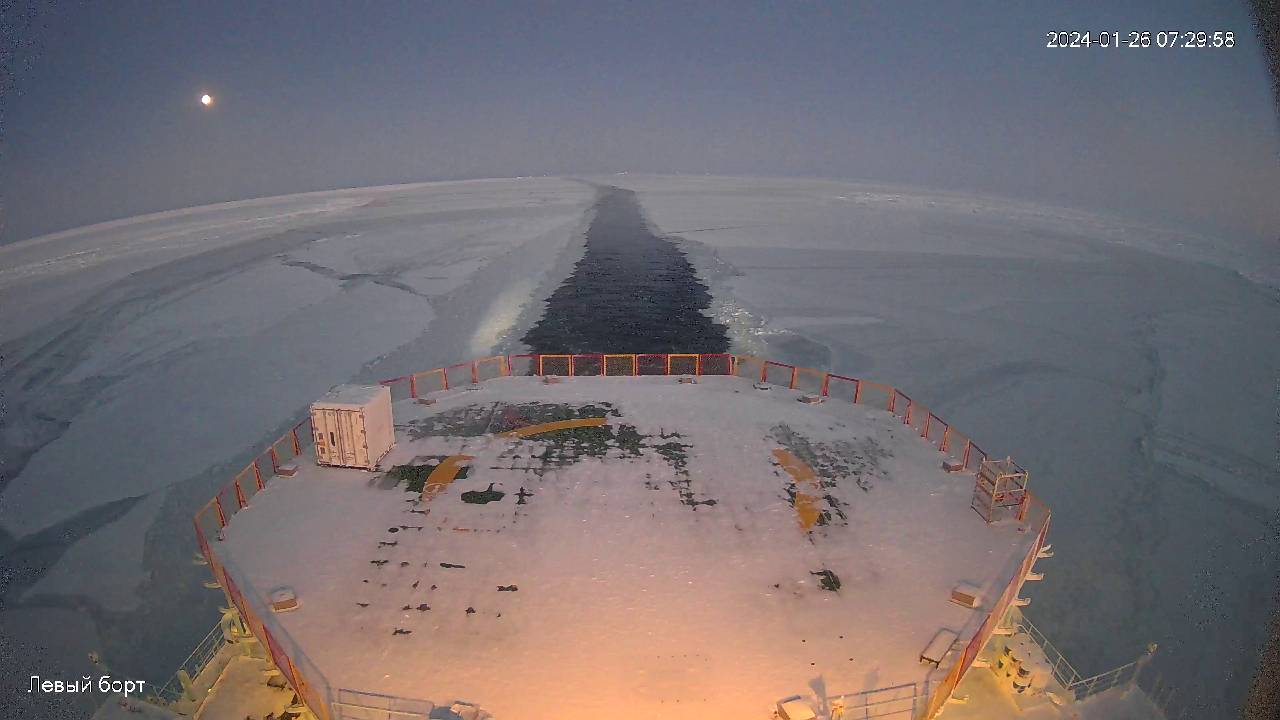
\includegraphics[scale=0.18]{src/Project_planning/assets/3920.jpg}}
    \subfloat[Ночной снимок]{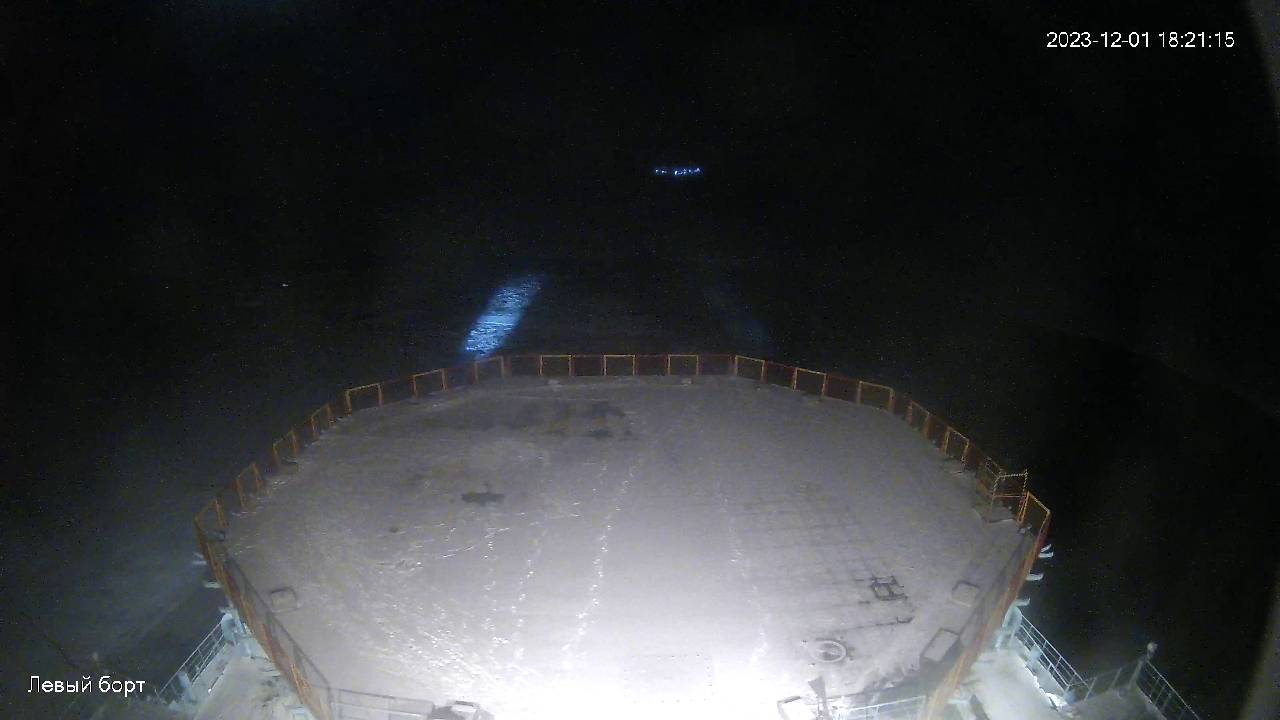
\includegraphics[scale=0.18]{src/Project_planning/assets/1145.jpg}}
    \caption{Примеры снимков кормовой камеры}\label{fig:camera_images}
\end{figure}

\subsection{Первый подход}
Поскольку в первом случае предполагалось использовать только средства уже установленные на ледокол, использовать глубокое обучение не представлялось возможным, 
так как никаких библиотек (Pytorch, TensorFlow и др) на ледоколе установлено не было. Это ставило ограничения на то, что первоначальный подход должен был 
использовать алгоритмы классического машинного обучения, а также техники компьютерного зрения, не использующие глубокое обучение.

Однако данный подход не ставил целью получения идеальной маски, так как был временным. Главной задачей первоначального подхода была разработка алгоритма, который 
мог бы выдавать маску канала, возможно сильно зашумленную, при ярком дневном освещении и при наличии в канале открытой воды.

\subsection{Второй подход}
Второй подход подразумевал возможность добавления на ледокол дополнительных библиотек, таких как Pytorch. Также ожидалось, что в комплекс помимо камеры, 
возможно будет включить тепловизор, что могло бы сильно облегчить задачу и сделать возможным наблюдение канала в ночное время суток, что особенно актуально зимой 
- в полярную ночь. Однако тепловизор так и не получилось включить в комплекс, из-за чего во второй части проекта всё также используется камера, но сам алгоритм 
уже реализован с использованием глубокого обучения.

Целью второго подхода, было создание алгоритма, способного выделять ледовый канал уже при более плохой видимости (в сумерках, в тумане, во время снегопада и т.д.), 
а также способный выделять ледовый канал покрытый ледяным салом (снегом и упавшим в него льдом). Данный подход уже не был скован узкими временными рамками, так как 
его установка на ледокол ожидается летом 2024 года.

\subsection{Общие ограничения}
\begin{figure}[htbp]
    \centering
    \subfloat[Заросший канал]{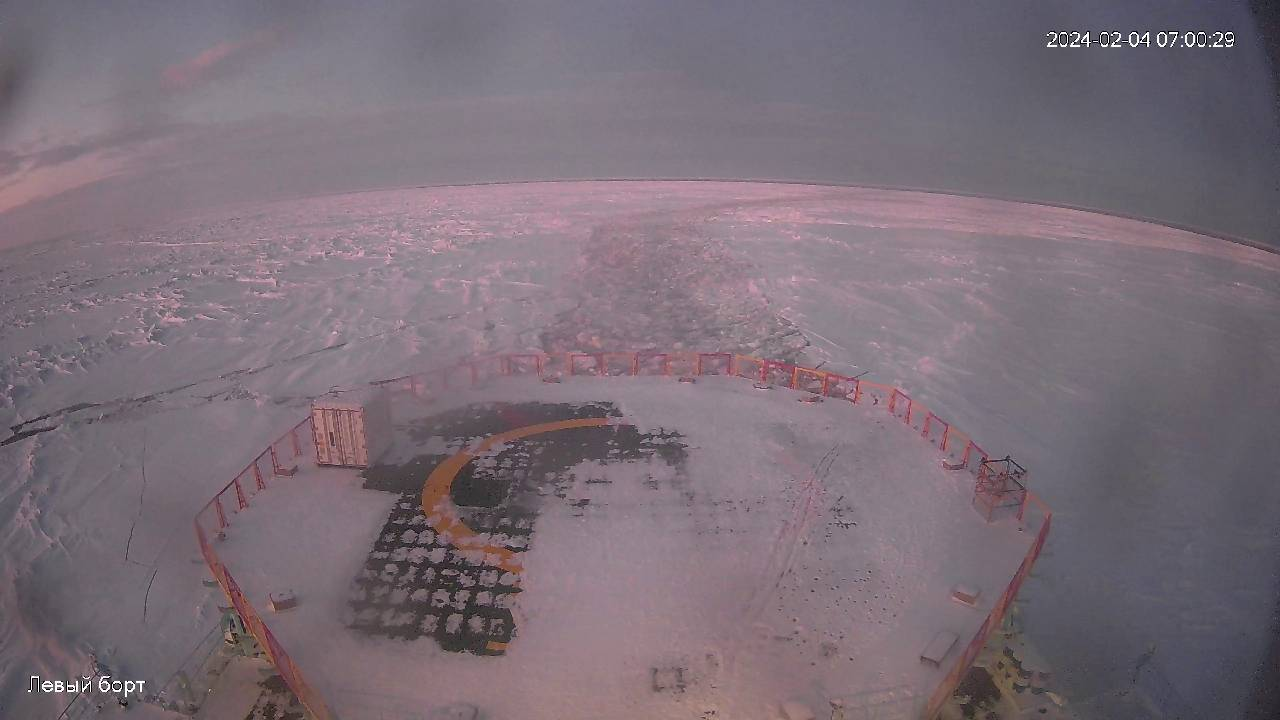
\includegraphics[scale=0.18]{src/Project_planning/assets/6513.jpg}}
    \subfloat[Канал, покрытый ледяным салом]{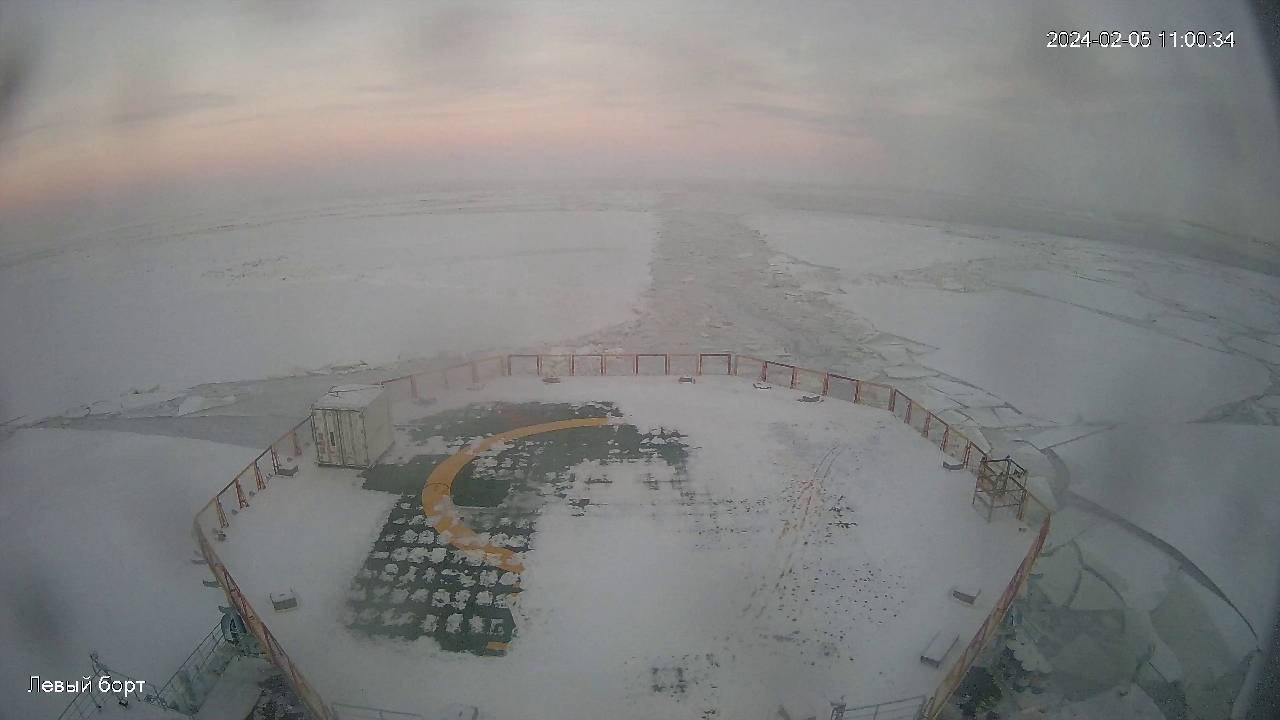
\includegraphics[scale=0.18]{src/Project_planning/assets/Заросший канал.jpg}}
    \caption{Сравнение кадров канала}\label{fig:closed channel}
\end{figure}
Оба описанных выше подхода также имеют некоторые общие ограничения.
\begin{enumerate}
    \item Отсутствие размеченных датасетов. Сейчас компьютерное зрение особенно сильно развивается в сфере автомобилей с автопилотом, в то время как для более специфических тем наработок немного. 
    Так как данный проект является первым в России (и, возможно, в мире), который ставит перед собой задачу анализа ледовой обстановки, 
    то не было возможности использовать какие-либо наработки в этой области в виду их отсутствия (по крайней мере в открытом доступе). В первую очередь это касается размеченных датасетов. 
    Это отразилось на методах, которые использовались во время работы.
    \item Сложность выделения ледового канала. Эта проблема отчасти связана с предыдущей. Выделять ледовый канал даже человеку порой бывает трудно, из-за чего результаты
    работы алгоритмов могут быть шумными, а также их оценка представляет собой нетривиальную задачу. На Рис.~\ref{fig:closed channel} представлены примеры канала. 
    Канал \textbf{a} уже зарос, в то время как канал \textbf{b} просто покрыт ледяным салом.
\end{enumerate} 

